% Dokumentace fykosích mp maker
% Lukáš Ledvina 10.2012 

\documentclass[a4paper,10pt]{article}

\usepackage{fkssugar}
\usepackage{xltxtra}
\usepackage{tabularx}
\usepackage{graphicx}
\usepackage{geometry}
\usepackage{ltablex}


\geometry{papersize={210mm,297mm},total={190mm,277mm}}

%\title{\texttt{Metapost}}
%\date{3. října 2012}

\begin{document}
%\maketitle
{\LARGE\centering FYKOSí {\tt MetaPost} --- dokumentace\\}\vspace{5mm}
\setcounter{section}{-1}
%%%%%%%%%%%%%%%%%%%%%%%%%%%%%%%%%%%%%%%%%%%%%%%%%
\section{Několik konvencí}
%%%%%%%%%%%%%%%%%%%%%%%%%%%%%%%%%%%%%%%%%%%%%%%%%
\begin{itemize}
\item Studujeme starší obrázky.
\item Body vyznačujeme pomocí \verb+odot(0.4mm,pozice)+.
\item Úhly kreslíme se základním poloměrem $"8 mm"$.
\item Šrafujeme s roztečí $"1 mm"$.
\end{itemize}

%%%%%%%%%%%%%%%%%%%%%%%%%%%%%%%%%%%%%%%%%%%%%%%%%
\section{Základní balíky}
%%%%%%%%%%%%%%%%%%%%%%%%%%%%%%%%%%%%%%%%%%%%%%%%%
{\centering\large\texttt{fks.mp}\nopagebreak\\\vspace{-12pt}\noindent}
\begin{tabularx}{\textwidth}{|l|l|X|}\hline
    kód & výsledek & použití\\\hline
    \verb+draw (0,0)--(u,0) dashed cerch+ & 
\includegraphics{mp_fks_1}& 
	čerchovaná čára\\\hline
    \verb+draw (0,0)--(u,0) dashed cark+ & 
\includegraphics{mp_fks_2}& 
	čárkovaná čára\\\hline
    \verb+draw (0,0)--(u,0) wp5+ & 
\includegraphics{mp_fks_3}& 
	použije 5x silnější pero\\\hline
    \verb+chpen5+ & 
\includegraphics{mp_fks_3}& 
	změní pero na 5x silnější\\\hline
    \verb+uhel(A,B,C,rad)+ & \raise-12pt\hbox{
\includegraphics{mp_fks_4}}& 
	nakreslí úhel $\sphericalangle ABC$ s obloučkem poloměru $"8 mm"$. 
	{\bf !TODO!} kreslit kruhový nikoli bezier.\\\hline
    \verb+uhelR(A,B,rad)+ & \raise-12pt\hbox{
\includegraphics{mp_fks_5}}& 
	nakreslí pravý úhel $\sphericalangle ABC$ s obloučkem 
	poloměru $"8 mm"$. Typicky se dělá menší než $"8 mm"$, zde $"5 mm"$.
	\\\hline
    \verb+axis((0,0),.2u,u,.1u,.5u)+ & \raise-12pt\hbox{
\includegraphics{mp_fks_6}}&
	osový kříž se středem v {\tt (0,0)}, dále rozsahy na osách\\\hline 
    \verb+srafuj((0,0)--(u,0)--(0,.5u)--cycle,dir45,1mm)+ & 
      \raise-12pt\hbox{
\includegraphics{mp_fks_7}}&
	šrafování, směr měníme dle potřeby, rozteč držíme na $"1 mm"$\\\hline 
    \verb+drawearrow+ & 
\includegraphics{mp_fks_8}&
	šipka s prázdnou hlavou\\\hline
    \verb+drawdblearrow+ & 
\includegraphics{mp_fks_9}&
	dvojitá šipka s prázdnou hlavou\\\hline
    \verb+drawvarrow+ & 
\includegraphics{mp_fks_10}&
	šipka s "V" hlavou\\\hline
    \verb+drawdblvarrow+ & 
\includegraphics{mp_fks_11}&
	dvojitá šipka s "V" hlavou\\\hline
    \verb+pruzina((0,0),(u,0),.2u,4)+ & 
\includegraphics{mp_fks_12}&
	pružinka se šířkou {\tt 0.2u} a čtyřmi závity\\\hline
    \verb+odot(.4mm,(0,0))+ & 
\includegraphics{mp_fks_13}&
	označení bodu, používá se {\tt 0.4mm}\\\hline
    \verb+kulicka(5mm,(0,0))+ & 
\includegraphics{mp_fks_14}&
	kulička\\\hline
    \verb+kotaDPK.ulft(z0,z1,0.5u,btex $l$ etex,0.5,0mm)+ &
	\raise-24pt\hbox{
\includegraphics{mp_fks_15}} & 
	kóta mezi body \verb+z0+ a \verb+z1+ odsazená o \verb+0.5u+ popisek 
	\verb+btex $l$ etex+ umístěný vlevo nahoru, posunutý na $50\%$ 
	k \verb+z1+, posunutý od dvojšipky o \verb+0mm+.\\\hline
    \verb+kotaDP.dir(poc,kon,lab,poz)+ &&
	\verb+kotaDPK.dir(poc,kon,0.5u,lab,poz,0mm)+\\\hline
    \verb+kotaD.dir(poc,kon,lab)+ &&
	\verb+kotaDP.dir(poc,kon,lab,0.5)+\\\hline
    \verb+kota(poc,kon,lab)+ &&
	\verb+kotaD.dir(poc,kon,lab)+, kde \verb+dir+ se nastavuje podle
	směru dvojšipky automaticky.\\\hline
    {\bf !TODO!} Zbylé kombinace&&\\\hline
    \verb+dist(a,b)+&&\\\hline
    \verb+provaz(size,path)+&\includegraphics{mp_fks_16}&Nakreslí lanko šířky
	\verb+size+ po trajektorii \verb+path+\\\hline
    \verb+provazVR(size,path)+&\includegraphics{mp_fks_17}&To samé, ale kreslí
	provaz, tj.~má vroubky. Jednotlibé provazy jdou na sebe navazovat, 
	při křížení cesty se může chovat nestandardně, mezní křivost je 
	\verb+1mm+ pro šířku 1 (platí přímá úměra).\\\hline
    \multicolumn{3}{|l|}{\emph{Další příkazy pocházejí z} {\tt fks-label.mp}}\\\hline
    \verb+olabel.poz(label,point)+ & & 
	standardní label, ale vykreslí též bod pomocí \verb+odot+, 
	který označuje\\\hline
    \verb+flabel.poz(label,point)+ & & 
	standardní label, ale vybílí kresbu pod sebou\\\hline
    \verb+oflabel.poz(label,point)+ & & 
	standardní label, superpozice výše uvedených\\\hline
    \multicolumn{3}{|l|}{\emph{Další příkazy pocházejí z} 
	{\tt mth-function.mp}}\\\hline
    \verb+sqr+  && druhá mocnina\\\hline
    \verb+log+  && desítkový logaritmus\\\hline
    \verb+ln+   && přirozený logaritmus\\\hline
    \verb+exp+  && exponenciála\\\hline
    \verb+inv+  && převrácená hodnota\\\hline
    \verb+pow+  && umocnění; (základ, exponent)\\\hline
    \hline
    \verb+sind+ && viz {\tt plain.mp}\\\hline
    \verb+cosd+ && viz {\tt plain.mp}\\\hline
    \verb+tand+ && tangens ve stupních\\\hline
    \verb+cotd+ && kotangens ve stupních\\\hline
    \verb+sin+  && sinus\\\hline
    \verb+cos+  && kosinus\\\hline
    \verb+tan+  && tangens\\\hline
    \verb+cot+  && kotangens\\\hline
    \hline
    \verb+sinh+ && hyperbolický sinus\\\hline
    \verb+cosh+ && hyperbolic kosinus\\\hline
    \verb+tanh+ && hyperbolický tangens\\\hline
    \verb+coth+ && hyperbolický kotangens\\\hline
    \hline
% inverse trigonometric and hyperbolic functions
    \verb+arcsind+ && inversní sinus ve stupních\\\hline
    \verb+arccosd+ && inversní kosinus ve stupních\\\hline
    \verb+arctand+ && inversní tangens ve stupních\\\hline
    \verb+arccotd+ && inversní kotangens ve stupních\\\hline
    \verb+arcsin+  && inversní sinus\\\hline
    \verb+arccos+  && inversní kosinus\\\hline
    \verb+arctan+ && inversní tangens\\\hline
    \verb+arccot+ && inversní kotangens\\\hline 
    \verb+argsinh+  && inversní sinus hyperbolický\\\hline
    \verb+argcosh+  && inversní kosinus hyperbolický\\\hline

    \verb+argtanh+  && {\bf !TODO!} inversní tangens hyperbolický\\\hline
    \verb+argcoth+  && {\bf !TODO!} inversní kotangens hyperbolický\\\hline
\end{tabularx}\bigskip

%%%%%%%%%%%%%%%%%%%%%%%%%%%%%%%%%%%%%%%%%%%%%%%%%
{\centering\large\texttt{fkscirc.mp}\nopagebreak\\\vspace{-12pt}\noindent}
\begin{tabularx}{\textwidth}{|l|l|X|}\hline
%\begin{longtable}{|l|l|p{8cm}|}\hline
    kód & výsledek & použití\\\hline
    \verb+fks_center:=true+ && přesun referenčního bodu součásky z konce 
	nožičky na optický střed. (Hotové pouze u níže dokumentovaných
	součástek.)\\\hline
    \verb+svorky+ & &\\\hline
    \verb+junction(z0)+ & & puntík na spojení vodičů.\\\hline
    \multicolumn{3}{|l|}{\emph{Další příkazy pocházejí z} {\tt makecirc-fks.mp}}\\\hline
    \verb+wire(z1,z2,type)+&&spojí dva body \verb+z1+ a \verb+z2+ vodičem,
	\verb+type+ $\in\{$\verb+nsq+ {\it pro přímé spojení\/}, \verb+udsq+ 
	{\it pro spoj začínající vodorovně\/}, \verb+rlsq+ {\it pro spoj 
	začínající svisle\/}$\}$\\\hline
    \verb+wireU(z1,z2,dist,type)+&&analogické, ale dělá U vodič vysunutý 
	o \verb+dist+. (Netestováno.)\\\hline
    \verb+inductor.La(z0,Up,45,name,val)+&
	\raise-12pt\hbox{\includegraphics{mp_circ_1}}&
	cívka, na pozici \verb+z0+, otočená o $"45\dg"$, \verb+Up, Down+ je 
	orientace kopečků. Dále definuje proměnné \verb+L.AA.l+ a \verb+L.AA.r+
	se souřadnicemi vývodů.\\\hline
    \verb+capacitor.Ca(z0,type,ang,name,val)+&
	\raise-12pt\hbox{\includegraphics{mp_circ_2}}&
	kondenzátor, dtto. volby: \verb+normal+, \verb+electrolytic+, 
	\verb+variable+ a \verb+variant+. Piny \verb+C.Ca.r+, \verb+C.Ca.l+.
\\\hline
    \verb+motor.Ma(z0,ang,name,val)+&
	\raise-12pt\hbox{\includegraphics{mp_circ_3}}&
	motor, dtto. Piny \verb+M.Ma.D+, \verb+M.Ma.B+\\\hline
    \verb+generator.Ga(...)+&&generátor, dtto. Piny \verb+G.Ga.B+ a 
	\verb+G.Ga.D+.\\\hline
    \verb+transformer.Ta(z0,type,ang)+&
	\raise-36pt\hbox{\includegraphics{mp_circ_4}}&
	trafo,\verb+type+ $\in\{$\verb+normal+ {\it normální}, 
	\verb+mid+ {\it s dvěma sekundáry}, \verb+Fe+ {\it takové veliké}, 
	\verb+auto+ {\it špatně definové piny}$\}$. Piny \verb+tr.Ta.pi+, 
	\verb+tr.Ta.ps+, \verb+tr.Ta.si+, \verb+tr.Ta.ss+ 
	a \verb+tr.Ta.m+.\\\hline
    \verb+source.Sa(z0,type,angle,name,val)+&
	\raise-24pt\hbox{\includegraphics{mp_circ_5}}&
	zdroj, dtto. Volby \verb+AC+, \verb+DC+, \verb+I+ a \verb+V+.  
	Piny: \verb+G.Ga.p+ a \verb+G.Ga.n+.\\\hline
    \verb+resistor+&&Nepoužívat --- americký vzor, nahrazen \verb+impedance+.
	\\\hline
    \verb+diode.Da(z0,type,ang,pin,name,val)+&
	\raise-12pt\hbox{\includegraphics{mp_circ_6}}&
	dioda, typ \verb+normal+, \verb+zener+ a \verb+LED+. Pin \verb+pinA+ 
	nebo \verb+pinK+ otáčí diodu o $"180\dg"$. Piny: \verb+D.Da.K+ a
        \verb+D.Da.A+.\\\hline
    \verb+transistor+&&{\bf !TODO!}\\\hline
    \verb+meains+&&{\bf !TODO!}\\\hline
    \verb+ground+&&{\bf !TODO!}\\\hline
    \verb+junction.ac(z0,"")(top)+&&puntík na spojení vodičů v bodě \verb+z0+.
	{\bf !TODO!} ostatní volby.\\\hline
%    \verb+impedance.Ra(z2,45,btex$R_1$etex,btex$"1\ohm"$etex)+&
    \verb+impedance.Ra(z2,45,name,val)+&
	\raise-12pt\hbox{\includegraphics{mp_circ_10}}&
	odpor s popiskem a velikostí v bodě \verb+z2+ otočený 
	o $"45\dg"$. Současně se vytvoří proměnné \verb+Ra.l+ a \verb+Ra.p+ se
	souřadnicemi konců vývodů. Nuté pro napojování vodičů. (verb bug)
	\\\hline
    \verb+lamp+&&{\bf !TODO!}\\\hline
    \verb+switch+&&{\bf !TODO!}\\\hline
    \verb+battery+&&{\bf !TODO!}\\\hline
    \verb+current+&&{\bf !TODO!}\\\hline
    \verb+imesh+&&{\bf !TODO!}\\\hline
    \verb+rheostat+&&{\bf !TODO!}\\\hline
\end{tabularx}\bigskip

%%%%%%%%%%%%%%%%%%%%%%%%%%%%%%%%%%%%%%%%%%%%%%%%%
{\centering\large\texttt{fks-3d.mp}\nopagebreak\\\vspace{-12pt}\noindent}
\begin{tabularx}{\textwidth}{|l|l|X|}\hline
    kód & výsledek & použití\\\hline
    \verb+VRP_tD+ && nastavení volného rovnoběžného promítání, 
	volá se na začátku.\\\hline
    \verb+AXON_tD+ && nastavení axonometrického promítání, 
	volá se na začátku.\\\hline
    \verb+PzP_tD+ && nastavení pohledu z prava (zobrazuje se rovina $yz$, 
	osa $x$ je opačná k ose $y$), volá se na začátku.\\\hline
    \verb+tD0=(2u,3u,1u)+ & & 3D proměnná analogická k {\tt z}.\\\hline
    \verb+dD?+   && pair s projektovanou hodnotou {\tt tD?}.\\\hline
    \verb+proj(x)+  && vrací pair s projekcí parametru\\\hline
    \verb+norm_tD?+  && norma {\tt tD?}\\\hline
    \verb+norm(x)+  && vrací velikost parametru\\\hline
    \verb+!part_tD?+  && vrací $!$-ovou složku {\tt tD?}; $!$ psán malým 
	písmenem\\\hline
    \verb+!part_tD?(x)+  && vrací $!$-ovou složku parametru; $!$ psán malým
        písmenem\\\hline
    \verb+x dotprod_tD y+  && vrací skalární součin $x$ a $y$\\\hline
    \verb+getTr(tD_o,tD_x,tD_y)+ && vrací transformaci z roviny definované body
	\verb+tD_o, tD_x, tD_y+ do projektivní roviny. Vhodné pro kreslení 
	křivek jež jsou ve 3D na nějaké rovině. \verb+tD_o+ je počátak 
	souřadnic na projektované rovině, \verb+tD_x+ směr osy $x$ a \verb+tD_y+
	další bod v projektované rovině (pomocí G-S OG se ortogonalizuje 
	k ose $x$).\\\hline
    \verb+shifted_dD(x)+ && transformace, jenž posouvá projektovaný bod 
	o 3D souřadnici $x$.\\\hline
    \verb+x SpRotate!_tD phi+ && otočí bod \verb+x+ o úhel \verb+phi+ kolem 
	osy \verb+!+ (psáno velkým písmenem)\\\hline
    \verb+rotate_tD(x,nP,nK,phi)+ && rotace x okolo normaloveho vektoru 
	nP$\to$nK o uhel phi\\\hline
\end{tabularx}\bigskip

%%%%%%%%%%%%%%%%%%%%%%%%%%%%%%%%%%%%%%%%%%%%%%%%%
\section{Loga -- grafika}
%%%%%%%%%%%%%%%%%%%%%%%%%%%%%%%%%%%%%%%%%%%%%%%%%
{\centering\large\texttt{fks-logo-color.mp}\nopagebreak\\\vspace{-12pt}\noindent}
\begin{tabularx}{\textwidth}{|l|l|X|}\hline
    kód & výsledek & použití\\\hline
    \verb+mpost fks-logo-color.mp+&
\includegraphics{fks-logo-color}& 
	barevný pták fykosák
{} {} {} {} {} {} {} {} {} {} {} {} {} {} {} {} {} {} {} {} {} {} {} {} {} {} {} {} {} {} {} {} {} {} {} {} {} {} {} {} {} {} {} {} {} {} {} {} {} {} {} {} {} {} {} {} {} {} {} {} {} {} {} {} {} {} {} {} {} {} {} {} {} {} {} {} {} {} {} {} {} {} {} {} {} {} {} {} {} {} {} {} {} {} {} {} {} {} {} {} {} {} {} {} {} {} {} {} {} {} {} {} {} {} {} {} {} {} {} {} {} {} {} {} {} {} {} {}
\\\hline
\end{tabularx}\bigskip

%%%%%%%%%%%%%%%%%%%%%%%%%%%%%%%%%%%%%%%%%%%%%%%%%
{\centering\large\texttt{fks-logo.mp}\nopagebreak\\\vspace{-12pt}\noindent}
\begin{tabularx}{\textwidth}{|l|l|X|}\hline
    kód & výsledek & použití\\\hline
    \verb+mpost fks-logo.mp+&
\includegraphics{fks-logo_1}& fks-logo.1
{} {} {} {} {} {} {} {} {} {} {} {} {} {} {} {} {} {} {} {} {} {} {} {} {} {} {} {} {} {} {} {} {} {} {} {} {} {} {} {} {} {} {} {} {} {} {} {} {} {} {} {} {} {} {} {} {} {} {} {} {} {} {} {} {} {} {} {} {} {} {} {} {} {} {} {} {} {} {} {} {} {} {} {} {} {} {} {} {} {} {} {} {} {} {} {} {} {} {} {} {} {} {} {} {} {} {} {} {} {} {} {} {} {} {} {} {} {} {} {} {} {} {} {} {} {} {} {}
\\\hline
    &
\includegraphics{fks-logo_2}& fks-logo.2\\\hline
    &
\includegraphics{fks-logo_3}& fks-logo.3\\\hline
    &
\includegraphics{fks-logo_4}& fks-logo.4\\\hline
    &
\includegraphics{fks-logo_5}& fks-logo.5\\\hline
    &
\includegraphics{fks-logo_6}& fks-logo.6\\\hline
    &
\includegraphics{fks-logo_7}& fks-logo.7\\\hline
    &
\includegraphics{fks-logo_8}& fks-logo.8\\\hline
    &
\includegraphics{fks-logo_9}& fks-logo.9\\\hline
    &
\includegraphics{fks-logo_10}& fks-logo.10\\\hline
    &
\includegraphics{fks-logo_11}& fks-logo.11\\\hline
    &
\includegraphics{fks-logo_12}& fks-logo.12\\\hline
\end{tabularx}\bigskip

%%%%%%%%%%%%%%%%%%%%%%%%%%%%%%%%%%%%%%%%%%%%%%%%%
{\centering\large\texttt{fks-tricko.mp}\nopagebreak\\\vspace{-12pt}\noindent}
\begin{tabularx}{\textwidth}{|l|l|X|}\hline
    kód & výsledek & použití\\\hline
    \verb+mpost fks-tricko.mp+ & 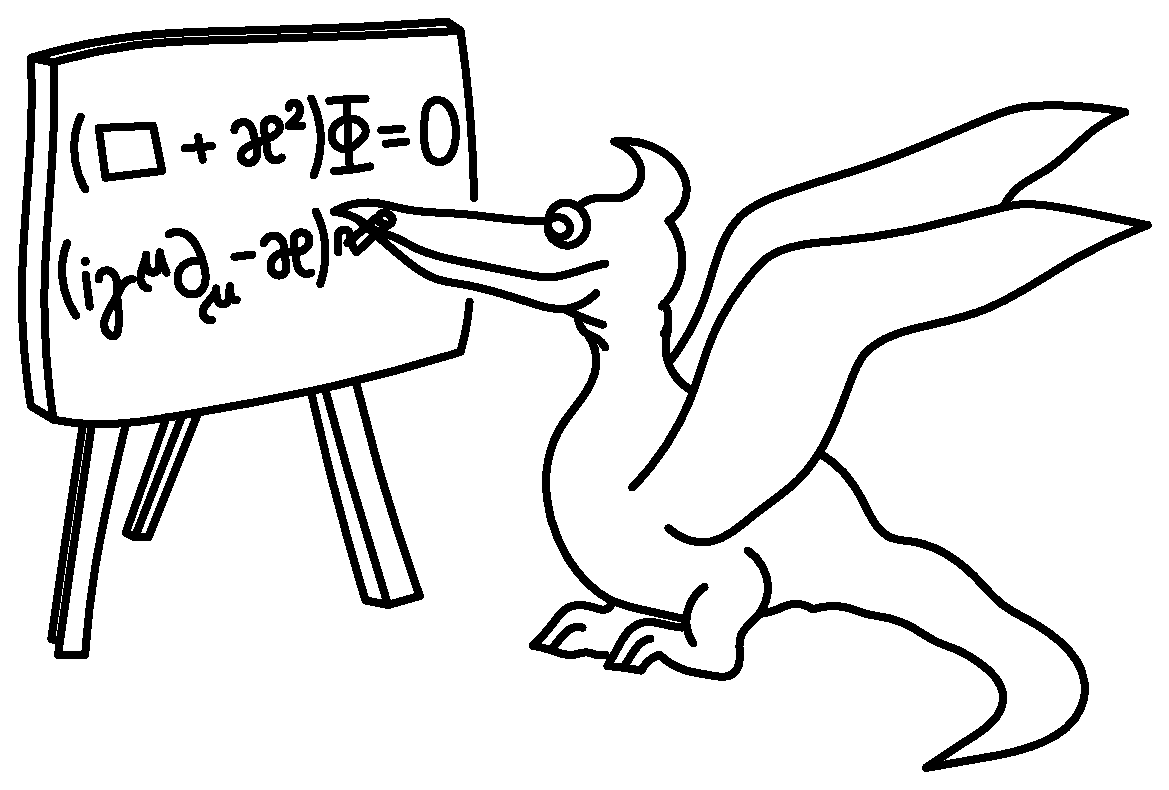
\includegraphics[width=3cm]{fks-tricko_1} & 
	fks-tricko.1
{} {} {} {} {} {} {} {} {} {} {} {} {} {} {} {} {} {} {} {} {} {} {} {} {} {} {} {} {} {} {} {} {} {} {} {} {} {} {} {} {} {} {} {} {} {} {} {} {} {} {} {} {} {} {} {} {} {} {} {} {} {} {} {} {} {} {} {} {} {} {} {} {} {} {} {} {} {} {} {} {} {} {} {} {} {} {} {} {} {} {} {} {} {} {} {} {} {} {} {} {} {} {} {} {} {} {} {} {} {} {} {} {} {} {} {} {} {} {} {} {} {} {} {} {} {} {} {}
\\\hline
    & 
\includegraphics[width=3cm]{fks-tricko_2} & fks-tricko.2\\\hline
\end{tabularx}\bigskip

%%%%%%%%%%%%%%%%%%%%%%%%%%%%%%%%%%%%%%%%%%%%%%%%%
\section{Nepoužívané balíky}
%%%%%%%%%%%%%%%%%%%%%%%%%%%%%%%%%%%%%%%%%%%%%%%%%
{\centering\large\texttt{fks-znacky.mp}\nopagebreak\\\vspace{-12pt}\noindent}
\begin{tabularx}{\textwidth}{|l|l|X|}\hline
    kód & výsledek & použití\\\hline
    Stará makra pro kreslení el. obvodů.&&
{} {} {} {} {} {} {} {} {} {} {} {} {} {} {} {} {} {} {} {} {} {} {} {} {} {} {} {} {} {} {} {} {} {} {} {} {} {} {} {} {} {} {} {} {} {} {} {} {} {} {} {} {} {} {} {} {} {} {} {} {} {} {} {} {} {} {} {} {} {} {} {} {} {} {} {} {} {} {} {} {} {} {} {} {} {} {} {} {} {} {} {} {} {} {} {} {} {} {} {} {} {} {} {} {} {} {} {} {} {} {} {} {} {} {} {} {} {} {} {} {} {} {} {} {} {} {} {}
\\\hline
\end{tabularx}\bigskip

%%%%%%%%%%%%%%%%%%%%%%%%%%%%%%%%%%%%%%%%%%%%%%%%%
{\centering\large\texttt{cary.mp}\nopagebreak\\\vspace{-12pt}\noindent}
\begin{tabularx}{\textwidth}{|l|l|X|}\hline
    kód & výsledek & použití\\\hline
    \verb+drawdots(size) path+ & 
\includegraphics{mp_cary_1} & 
	kolečko s otvorem v každém řídícím bodu křivky\\\hline
    \verb+drawhlines(size) path+ & 
\includegraphics{mp_cary_2}&
	vodorovná čárka, dtto.\\\hline
    \verb+drawvlines(size) path+ & 
\includegraphics{mp_cary_3}&
	svislá čárka, dtto.\\\hline
    \verb+drawctverce(size) path+ & 
\includegraphics{mp_cary_4}&
	čtverce, dtto.\\\hline
    \verb+drawtrojuhelniky(size) path+ & 
\includegraphics{mp_cary_5}&
	trojúhleníky, dtto.\\\hline
    \verb+drawkosoctverce(size) path+ & 
\includegraphics{mp_cary_6}&
	kosočtverce, dtto.
{} {} {} {} {} {} {} {} {} {} {} {} {} {} {} {} {} {} {} {} {} {} {} {} {} {} {} {} {} {} {} {} {} {} {} {} {} {} {} {} {} {} {} {} {} {} {} {} {} {} {} {} {} {} {} {} {} {} {} {} {} {} {} {} {} {} {} {} {} {} {} {} {} {} {} {} {} {} {} {} {} {} {} {} {} {} {} {} {} {} {} {} {} {} {} {} {} {} {} {} {} {} {} {} {} {} {} {} {} {} {} {} {} {} {} {} {} {} {} {} {} {} {} {} {} {} {} {}
\\\hline
\end{tabularx}\bigskip
\end{document}
